\documentclass[border=10pt]{standalone}

\usepackage{tikz}
\usepackage{tikzsymbols}
\usetikzlibrary{calc,patterns,shapes.geometric}

\def\centerarc[#1](#2)(#3:#4:#5){\draw[#1] ($(#2)+({#5*cos(#3)},{#5*sin(#3)})$) arc (#3:#4:#5);}

\begin{document}
	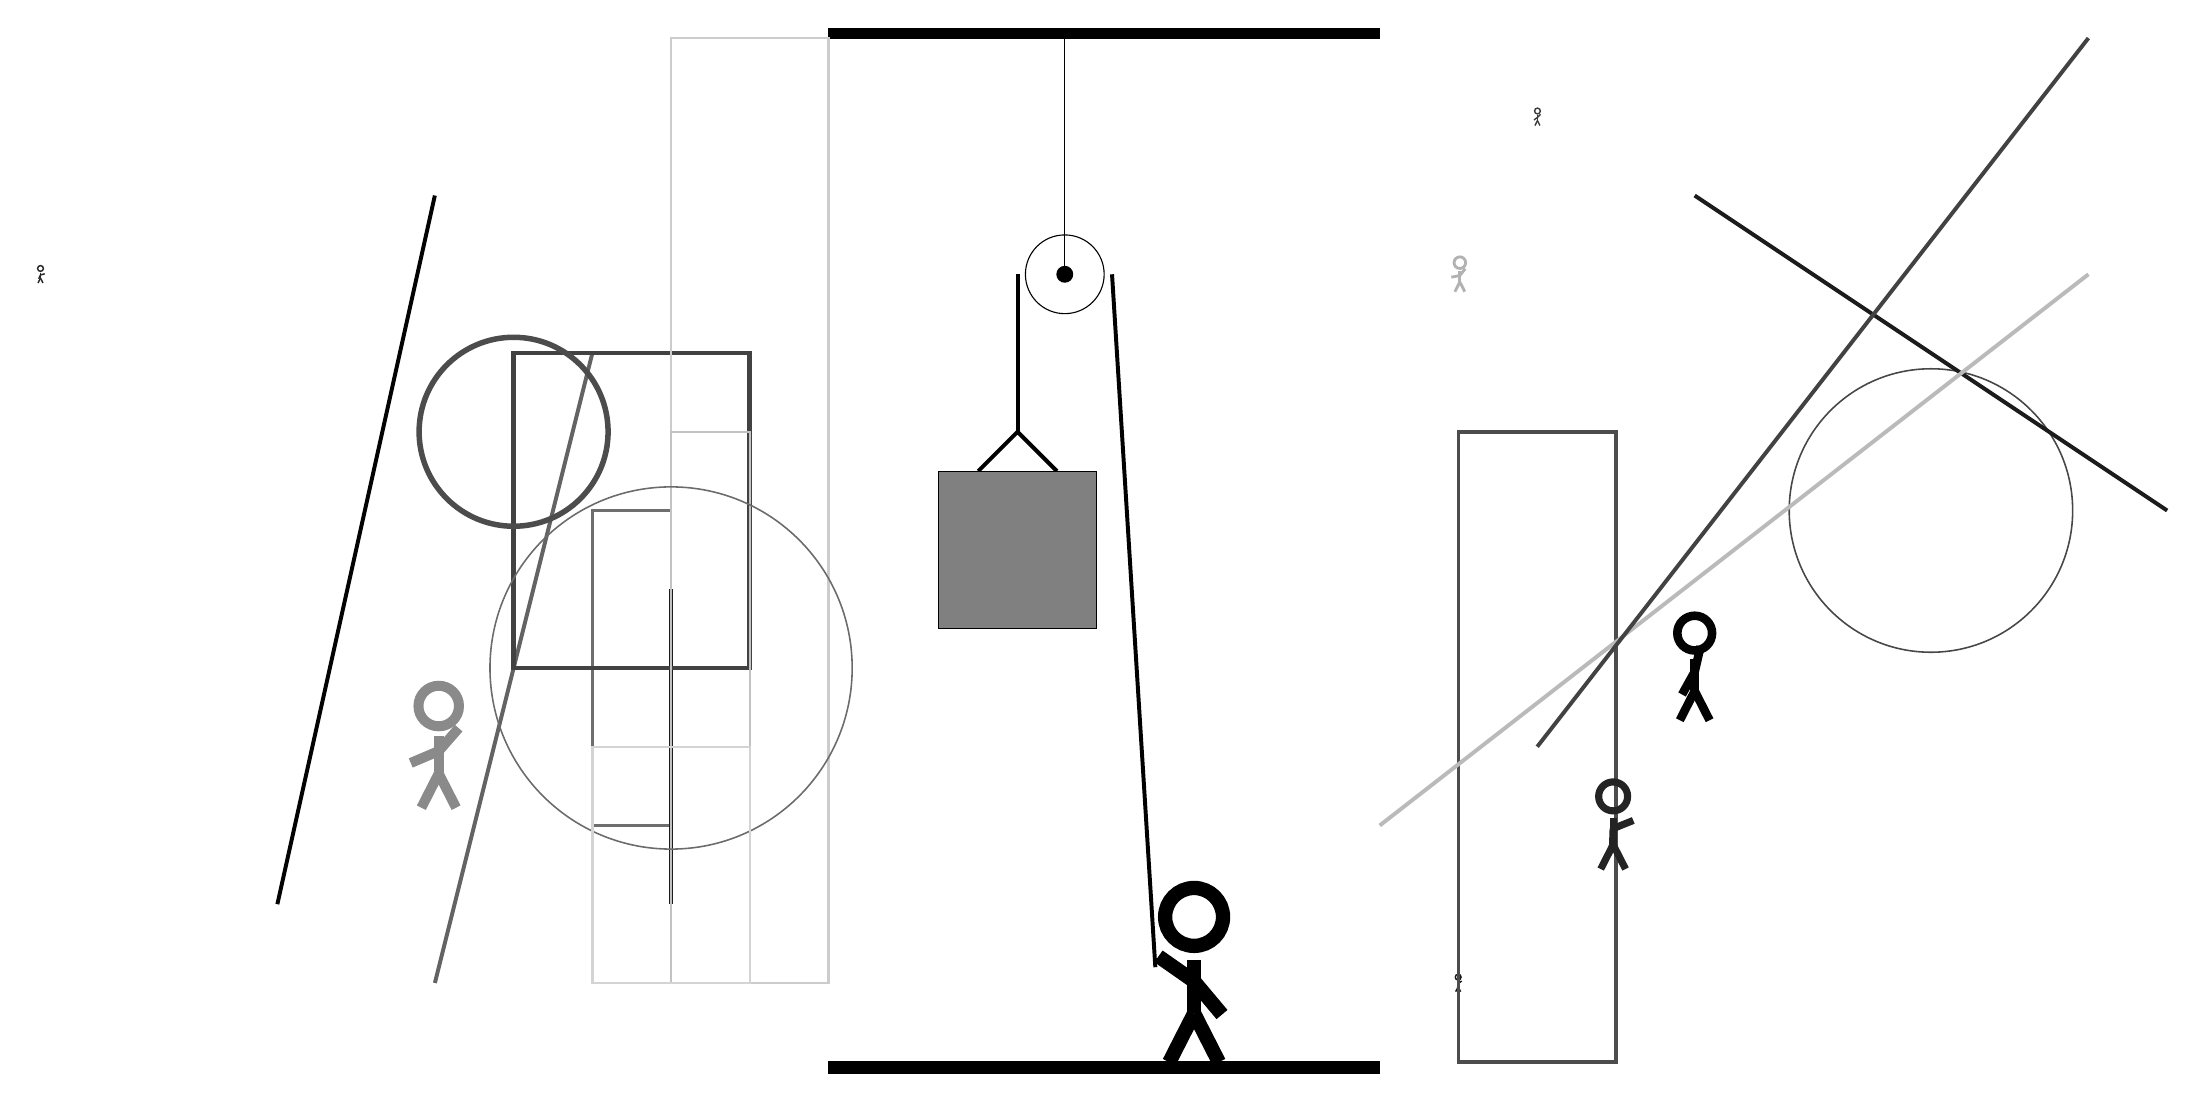
\begin{tikzpicture}
		%%%%% START %%%%%
		
		\draw[fill=black] (-2, 10) rectangle (5, 10.125);
		
		\draw (1, 7) circle (0.5);
		\draw[fill=black] (1, 7) circle (0.1);
		\draw (1, 10) -- (1, 7);
		
		\draw[line width=0.5mm] (-0.1, 4.5) -- (0.4, 5.0) -- (0.9, 4.5);
		\draw[fill=black!50] (-0.6, 4.5) rectangle (1.4, 2.5);
		
		\draw[line width=0.5mm] (0.4, 7) -- (0.4, 5.0);
		\centerarc[line width=0.5mm](1, 7)(0:180:0.6);
		\draw[line width=0.5mm](1.6, 7) -- (2.15, -1.8);
		
		\node[line width=0.3mm, color=black!91] at (6, -2) {\Strichmaxerl[1][82][36]};
		
		\draw[line width=0.3mm, color=black!57] (-4, 0) rectangle (-5, 4);
		\draw [line width=0.2mm, color=black!72](12, 4) circle (1.8);
		\node[line width=0.2mm, color=black!46] at (-7, 1) {\Strichmaxerl[7][23][49]};
		\draw[line width=0.5mm, color=black!61](-7, -2) -- (-5, 6);
		\draw[line width=0.5mm, color=black!89](-4, -1) -- (-4, 3);
		
		\draw[line width=0.5mm, color=black!70] (6, -3) rectangle (8, 5);
		\draw[line width=0.6mm, color=black!74] (-3, 6) rectangle (-6, 2);
		\node[line width=0.2mm, color=black!85] at (-12, 7) {\Strichmaxerl[1][65][14]};
		\draw[line width=0.5mm, color=black!99](-7, 8) -- (-9, -1);
		\draw[line width=0.3mm, color=black!20] (-2, 10) rectangle (-4, -2);
		\draw [line width=0.7mm, color=black!70](-6, 5) circle (1.2);
		\node[line width=0.6mm, color=black!77] at (7, 9) {\Strichmaxerl[1][36][46]};
		\node[line width=0.2mm, color=black!86] at (8, 0) {\Strichmaxerl[5][88][22]};
		\draw[line width=0.3mm, color=black!24] (-4, -2) rectangle (-3, 5);
		\draw[line width=0.5mm, color=black!89](9, 8) -- (15, 4);
		\draw[line width=0.5mm, color=black!27](5, 0) -- (14, 7);
		\draw[line width=0.5mm, color=black!74](7, 1) -- (14, 10);
		\node[line width=0.6mm, color=black!99] at (9, 2) {\Strichmaxerl[6][61][77]};
		\draw [line width=0.2mm, color=black!58](-4, 2) circle (2.3);
		\draw[line width=0.3mm, color=black!17] (-3, -2) rectangle (-5, 1);
		
		\node[line width=0.5mm, color=black!30] at (6, 7) {\Strichmaxerl[2][11][52]};
		
		\node at (2.6, -1.9) {\Strichmaxerl[10][-35][-50]};
		
		\draw[fill=black] (-2, -3) rectangle (5, -3.15);
		
		%%%%% END %%%%%
	\end{tikzpicture}
\end{document}